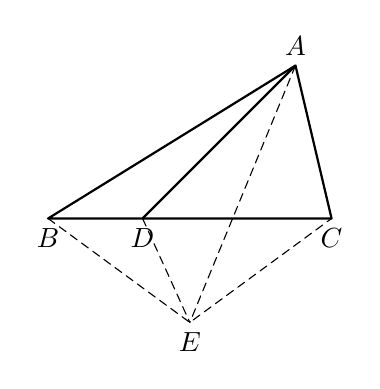
\begin{tikzpicture}[line cap=round,line join=round,scale=0.6]
\pgfmathsetmacro{\sfive}{sqrt(5)}

\coordinate (B) at (-3,0);
\coordinate (C) at (3,0);
\coordinate (D) at (-1,0);
\coordinate (A) at (\sfive,{1+\sfive});

% E 取在下方（示意折叠后的点）
\coordinate (E) at (0,-2.2);

\draw[thick] (B)--(C)--(A)--cycle;
\draw[thick] (A)--(D);

\draw[densely dashed] (B)--(E)--(C);
\draw[densely dashed] (D)--(E);
\draw[densely dashed] (A)--(E);

\node[below] at (B) {$B$};
\node[below] at (D) {$D$};
\node[below] at (C) {$C$};
\node[above] at (A) {$A$};
\node[below] at (E) {$E$};
\end{tikzpicture}